%
% Abschlussarbeit mit LaTeX
% ===========================================================================
% This is part of the book "Abschlussarbeit mit LaTeX".
% Copyright (c) 2002, 2003, 2005 Tobias Erbsland, Andreas Nitsch
% See the file main.tex for copying conditions.
%

\chapter{Konfiguration}
\index{Konfiguration}

\section{MiKTeX}
\index{Konfiguration!MiKTeX}

Die \DMLLaTeX"=Distribution \enquote{MiKTeX} musst du nicht konfigurieren. Es handelt sich dabei außer bei dem DVI-Betrachter um Kommandozeilentools. Du solltest nur den Editor TeXnicCenter einrichten (siehe dazu \cref{sec:KonfigurationTeXnicCenter}).

Du solltest jedoch mit dem \enquote{MiKTeX Update Wizard} alle Pakete der Distribution auf den neuesten Stand bringen. Wie du das machst, beschreibt die Hilfe zu MiKTeX ausführlich.\footnote{\enquote{User Guide}$\Rightarrow$\enquote{Maintenance}$\Rightarrow$\enquote{Installing Updates}}

\section{TeXnicCenter}
\label{sec:KonfigurationTeXnicCenter}
\index{Konfiguration!TeXnicCenter}

\subsection{TeXnicCenter für die Verwendung mit MiKTeX konfigurieren}

Nach dem ersten Start erscheint der Einrichtungsassistent. Falls du diesen bereits abgebrochen hast, kann man ihn über das Menü \enquote{Ausgabe}, \enquote{Ausgabeprofile definieren...} und dort in dem Dialog \enquote{Assistent} links unten erneut aufrufen. Doch wie schon gesagt, der Assistent startet normalerweise beim ersten Start vom TeXnicCenter automatisch.

\begin{figure}[hb]
	\begin{captionbeside}[Start des Konfigurations-Assistenten]{Der Konfigurationsassistent  startet mit diesem Screen.}[l]
		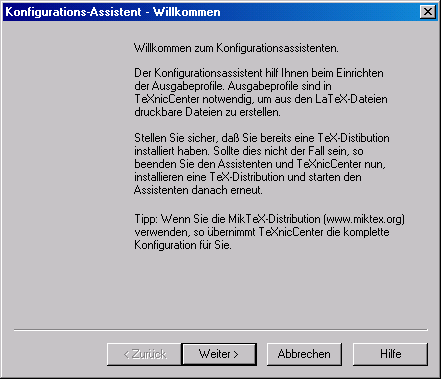
\includegraphics[width=7cm]{images/konfiguration01.png}
	\end{captionbeside}
	\label{fig:konfiguration01}
\end{figure}

\begin{figure}[hb]
	\begin{captionbeside}[Frage, für welche Distribution TeXnicCenter eingerichtet werden soll]{Hier teilt der Installations"=Assistent mit, dass die installierte MiKTeX"=Distribution erkannt wurde und fragt, ob er den Editor mit dieser \DMLLaTeX"=Distribution konfigurieren soll. Du wählst natürlich \enquote{Ja}.}[l]
		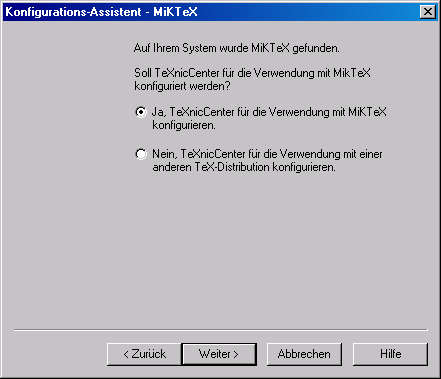
\includegraphics[width=7cm]{images/konfiguration02.png}
	\end{captionbeside}
	\label{fig:konfiguration02}
\end{figure}

\begin{figure}[ht]
	\begin{captionbeside}[Optionale Eingabe eines Postscript Betrachters]{Jetzt wirst du nach einem Programm zur PostScript-Betrachtung gefragt. Hier lässt du alle Felder leer.}[l]
		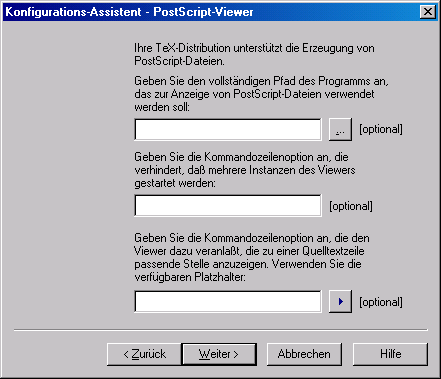
\includegraphics[width=7cm]{images/konfiguration03.png}
	\end{captionbeside}
	\label{fig:konfiguration03}
\end{figure}

\begin{figure}[ht]
	\begin{captionbeside}[Anzeige der drei generierten Profile]{Der TeXnicCenter-Assistent teilt dir mit, dass er drei Profile generieren wird. Ein DVI-, ein PostScript- und ein PDF-Profil. Wir werden nur das PDF-Profil verwenden.}[l]
		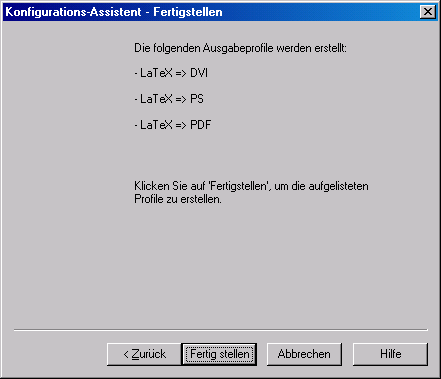
\includegraphics[width=7cm]{images/konfiguration04.png}
	\end{captionbeside}
	\label{fig:konfiguration04}
\end{figure}

\clearpage % Warten auf alle Floats

\subsection{Die Rechtschreibprüfung}
\index{Rechtschreibprufung@Rechtschreibprüfung}

Ein sehr nützliches Feature, welches dir TeXnicCenter bietet, ist die Rechtschreibprüfung. Wähle dazu im Menü \emph{Extras} den Punkt \emph{Optionen} aus. In dem Dialog, der sich öffnet, wählst du den Reiter \emph{Rechtschreibung} aus. Dort kannst du die verschiedenen Optionen der Rechtschreibprüfung einstellen, wie du in \cref{fig:rechtschreibung} siehst.

\begin{figure}
	\centering
		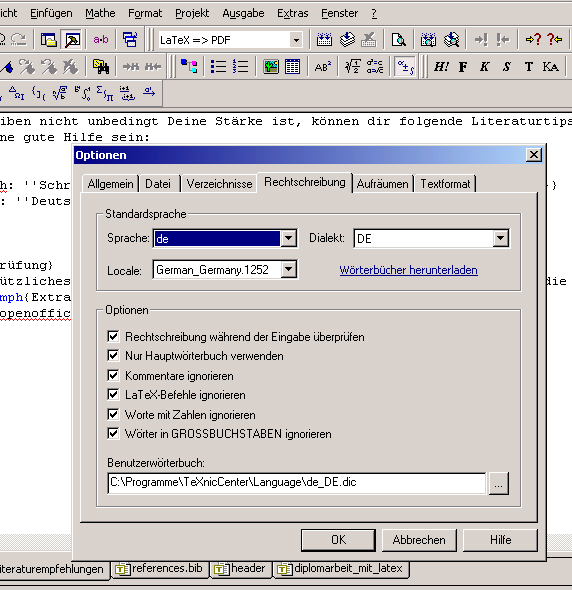
\includegraphics[width=0.60\textwidth]{images/rechtschreibung.png}
	\caption{Konfigurationsmöglichkeiten der Rechtschreibprüfung}
	\label{fig:rechtschreibung}
\end{figure}

Falls eine gewünschte Sprache fehlt, findest du Wörterbücher weiterer Sprachen unter
\urlindent{https://extensions.services.openoffice.org/dictionaries}
zum kostenlosen Download. Entpacke die in der heruntergeladenen ZIP"=Datei enthaltenen Dateien in das Unterverzeichnis \enquote{Language} deiner TeXnicCenter"=Installation, normalerweise ist das:

\verb|C:\Programme\TeXnicCenter\Language|.
